\documentclass[11pt]{article}
\usepackage[a4paper,margin=22mm,headheight=16pt]{geometry}
\usepackage{fontspec,xeCJK,xcolor,graphicx,enumitem,fancyhdr,titlesec}
\usepackage{hyperref}
\IfFontExistsTF{Times New Roman}{\setmainfont{Times New Roman}}{\setmainfont{TeX Gyre Termes}}
\IfFontExistsTF{FangSong}{\setCJKmainfont[AutoFakeBold=2]{FangSong}}{\IfFontExistsTF{仿宋}{\setCJKmainfont[AutoFakeBold=2]{仿宋}}{\IfFontExistsTF{FandolFang-Regular.otf}{\setCJKmainfont[AutoFakeBold=2]{FandolFang-Regular.otf}}{\setCJKmainfont{FandolSong-Regular.otf}}}}
\definecolor{ink}{HTML}{173747}\definecolor{accent}{HTML}{227E82}
\hypersetup{colorlinks=true,urlcolor=accent,linkcolor=accent}
\linespread{1.22}\setlength{\parindent}{0pt}\setlength{\parskip}{6pt}
\setlist[itemize]{leftmargin=1.4em,itemsep=3pt}
\titleformat{\section}{\large\bfseries\color{ink}}{}{0pt}{}
\titlespacing*{\section}{0pt}{14pt}{7pt}
\pagestyle{fancy}\fancyhf{}\lhead{\small OMNI LEARNING / 学习手册}\rhead{\small 有来源的学习}\cfoot{\small\thepage}
\emergencystretch=2em\widowpenalty=10000\clubpenalty=10000
\newcommand{\Needspace}[1]{\par\begingroup\dimen0=#1\relax\vskip0pt plus\dimen0\penalty-100\vskip0pt plus-\dimen0\vskip\dimen0\penalty9999\vskip-\dimen0\vskip0pt\endgroup}
\begin{document}


{\LARGE\bfseries\color{ink} 工作流与Agent如何选择}\par

2026-11-25 | Day02/30 | 阅读 8 分钟 + 练习 3 分钟\par\vspace{6pt}

\Needspace{5\baselineskip}\section*{今日导航}

今天回答：步骤多，就一定需要自主 Agent 吗？目标是用任务不确定性、可验证性和成本解释架构取舍。先用一分钟复述昨日旅行助手的完成条件，保留它作为今天的共同案例。

\Needspace{5\baselineskip}\section*{相同目标可以有不同路径}

假设目标是整理发票：文件类型固定、字段固定、规则明确。预设“读取—提取—校验—汇总”通常更容易控制。假设目标是调查一次旅行计划为何无法满足限制，系统可能需要根据查询结果调整方向。二者都能用到模型，差异在于谁决定下一步。[S1]

沿下排的返回箭头走一圈，再找出允许退出循环的那条分支。

\begin{center}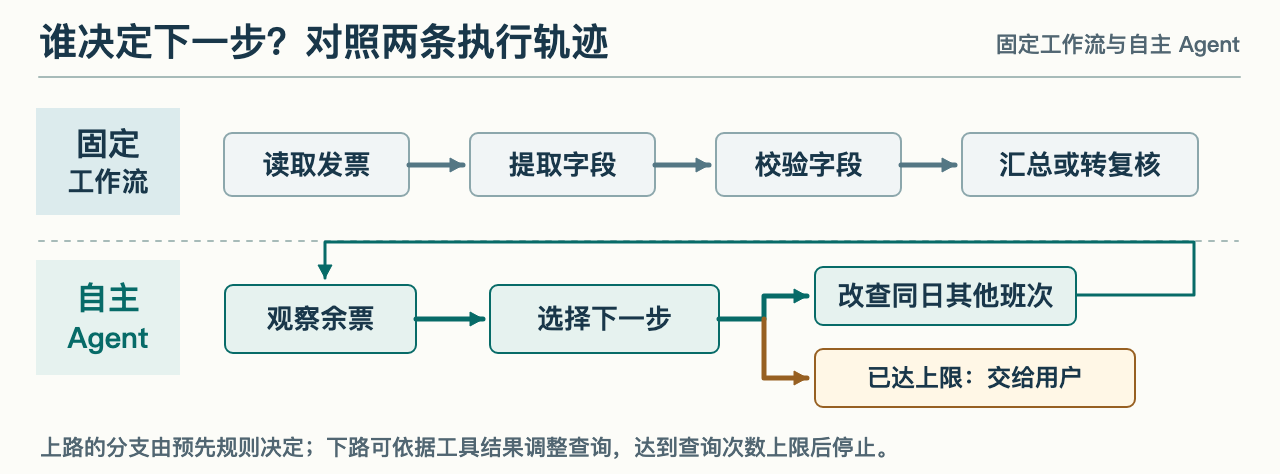
\includegraphics[width=\linewidth,height=0.26\textheight,keepaspectratio]{../assets/figure-db6bcab83918.png}\par

{\small 固定流程与可回看的查询循环 哪条路线会根据新的余票结果重新决定下一步？ 下路从改查班次返回观察节点；到达查询上限时转交用户。上路的汇总或复核已在校验规则中指定。 [S1]}\par

{\footnotesize 原创结构对照；发票与余票案例取自本课教学设计。}\end{center}

\Needspace{5\baselineskip}\section*{工作流与反馈循环}

工作流把主要路径预先规定好，模型可以参与其中某些步骤；Agent 的下一步更依赖当前观察与模型决策。上排的发票校验分支在设计时已经规定，下排则允许根据查询结果重新选路。循环本身不保证更聪明，它也会放大错误和耗时。

产品取舍可从三个问题开始：输入变化多不多？失败能否明确识别？额外探索是否带来足够收益？若任务本来一次调用就能完成，增加多个代理和循环可能只增加等待。Anthropic 建议从能满足需要的简单方案出发，并指出自主性常伴随时延与成本取舍。[S1]

Google ADK 的分类进一步说明，顺序或循环编排也可以被框架称为 workflow agents。[S5] 因此面试时先定义你采用的术语，再解释实际控制方式，避免双方用同一个词讨论不同东西。

\Needspace{5\baselineskip}\section*{旅行助手的混合设计}

一种教学设计是：固定收集日期与预算，模型负责识别偏好；查询候选走可检查的工具调用；当没有合适候选时，允许模型提出调整方向，但要求用户确认放宽哪一条条件。最终提交仍走固定确认步骤。

这一方案把灵活性放在确实需要判断的地方，把不可省略的检查留在稳定环节。停止条件也要明确：达到查询次数或时间预算仍找不到方案，就总结已尝试条件并请求用户选择。不要把“再想想”作为无限重试策略。评价时比较任务达成、等待时间和需要纠错的比例，而不是比较代理数量。[S3]

\Needspace{5\baselineskip}\section*{三分钟练习与自查}

把三个任务分别选为“单次调用”“固定工作流”“带反馈的 Agent”，并写一句理由：把一句话译成英文；按公司固定模板汇总报销；调查一个资料不全的问题并决定下一步搜什么。

参考选择依次如上，但实际边界取决于输入和质量要求。追问：若公司模板频繁变化，是否立即改成完全自主？不一定，可以先改善模板配置与校验。自查时确认你的理由来自任务特征，而非“Agent比较先进”。

\Needspace{5\baselineskip}\section*{复盘与明日连接}

自主性是一种设计选择，需要用收益解释其成本。一个可用产品往往混合固定规则、模型判断和人工确认。明天继续旅行案例：当工具能读写真实系统时，权限和确认应放在哪里？

\Needspace{6\baselineskip}\section*{扩展学习（选读）}\small 以下为选读，不计入每日必做时间。\begin{enumerate}[leftmargin=1.6em]

\item [S1] \href{https://www.anthropic.com/engineering/building-effective-agents}{Building effective agents} — 读工作流与 Agent 的区分；用作架构框架，不把旧工具清单当最新。\par Anthropic | 发布: 2024-12-19 | 核验: 2026-11-25

\item [S2] \href{https://www.anthropic.com/engineering/writing-tools-for-agents}{Writing effective tools for agents} — 关注工具边界、返回结果和评价方法如何影响可用性。\par Anthropic | 发布: 2025-09-11 | 核验: 2026-11-25

\item [S3] \href{https://www.anthropic.com/engineering/demystifying-evals-for-ai-agents}{Demystifying evals for AI agents} — 理解结果评价与执行轨迹；为后续验收指标课程准备。\par Anthropic | 发布: 2026-01-09 | 核验: 2026-11-25

\item [S4] \href{https://modelcontextprotocol.io/specification/2025-06-18}{Model Context Protocol specification} — 阅读指定版本的用途和安全原则；不称其为最新版本。\par MCP project | 发布: 2025-06-18（指定版本） | 核验: 2026-11-25

\item [S5] \href{https://adk.dev/agents/}{Agents in ADK} — 比较 LLM Agent、工作流 Agent 与自定义 Agent 的分类。\par Google ADK | 发布: 未标注 | 核验: 2026-11-25

\end{enumerate}

\end{document}